\documentclass[../proyecto.tex]{memoir}

\begin{document}

\chapter{Aproximación conceptual}

En este capítulo daremos una descripción conceptual del universo del juego de vida de Conway, junto con la descripción del juego de vida de Conway $\alpha$-asíncrono. Con éste contexto, se describirán en qué han consistido las simulaciones y sobre qué configuraciones iniciales se han realizado.

\section{Juego de vida de Conway}

Una configuración del juego de vida de Conway es la disposición sobre la malla de un conjunto de células. Por tanto una configuración inicial hace referencia a la disposición inicial de células sobre las que aún no se han aplicado las reglas de evolución. De esta manera cada nodo de la malla tiene dos estados posibles: vacío (0) o  ocupado (1). 

Las reglas de evolución que se aplican en cada iteración simultáneamente a todos los nodos de la malla son las siguientes:
\begin{itemize}
\item Un nodo ocupado se mantiene así si en su vecindario tiene solamente dos o tres nodos ocupados, en otro caso el nodo se vacía.
\item Un nodo vacío se ocupa cuando en su vecindario hay exactamente tres nodos, en otro caso mantiene su estado vacío.
\end{itemize}
Usualmente se consideran como pertenecientes al vecindario los nodos adyacentes en las direcciones horizontal, vertical y diagonales. 

En lo que hemos interpretado como un sentido \textit{biológico}, las reglas se pueden describir también interpretando los nodos ocupados como células vivas y la configuración inicial como una población de células:
\begin{itemize}
\item Una célula puede \textit{morir de soledad}, es decir, tiene solamente una célula en su vecindario o por \textit{superpoblación}, esto es, tiene cuatro o más células en su vecindario.
\item En un nodo vacío \textit{nace} una célula si en su vecindario hay exactamente tres células vivas.
\end{itemize}

La elección de las reglas de evolución parecería \textit{a priori} aleatoria, sin embargo, Conway las escogió aplicando las siguientes pautas \cite{libroGardner}:
\begin{itemize}
	\item No debe existir una disposición inicial de células para la cual haya una \textit{prueba simple} de que la población crezca sin límite. Esto es, no debe de ser posible predecir fácilmente la evolución de una configuración inicial.
	\item Debe haber disposiciones iniciales de células que aparentemente crezcan sin límite. 
	\item Debe haber disposiciones iniciales de células \textit{sencillas} que crezcan y cambien durante un periodo relativamente largo, llegando a tres posibles finales: desaparecer completamente ya sea debido a superpoblación o a dispersión, estabilizarse en una configuración que se mantenga constante o entrar en un ciclo sin fin de oscilación.
\end{itemize}

Sin embargo las reglas que proporcionó Conway no son las únicas que muestran evoluciones interesantes. La siguiente notación nos es útil para expresar distintas reglas de evolución abreviadamente. La reglas de evolución vienen dadas en la forma \textit{Bx/Sy} donde \textit{y} define el número de nodos ocupados en el vecindario para que un nodo ocupado se mantenga y \textit{x} el número de nodos ocupados en el vecindario para que un nodo vacío se ocupe. Por ejemplo, para el juego de vida es B3/S23. Destacamos la regla B1357/S1357 conocida como \textit{Edward Fredkin's replicating automaton}, en la cual cada configuración es eventualmente reemplazada por múltiples copias de sí misma, la regla B3/S12345 conocida como \textit{Maze}, genera configuraciones similares a laberintos, una variación muy curiosa es que si añadimos el número 7 a la parte \textit{B} es posible observar como un nodo ocupado recorre el laberinto y la regla B3/S012345678 conocida como \textit{Life without Death}, en la cual los nodos ocupados nunca se vacían, se caracteriza por un crecimiento caótico y la aparición de configuraciones similares a escaleras que pueden ser usadas para simular circuitos booleanos \cite{regla1}.

%Estaría muy bien añadir imágenes aquí pero me va a tomar un ratete hacerlo.

%Fijada una configuración inicial $z$, enteremos por ejecución o simulación del juego de vida de Conway de duración $n \in \mathds{N} \cup \{ \infty\}$ al resultado de aplicar $n$ veces la función de transición global del juego de vida de Conway a la configuración inicial y lo notaremos $C_{n}(z)$. Sea $t$ tal que $1 \leq t \leq n$, diremos que es el instante $t$ de la ejecución/simulación/experimento del juego de vida de Conway de duración $t$, el resultado de aplicar $t$ veces la función de transición global a una configuración inicial $z$ y lo notaremos $C^t_n(z)$. Por último, los conjuntos de puntos $C^{t'}_{n'}(z')$, $C^{t}_{n}(z)$ si los conjuntos de células de cada simulación son idénticos. De la misma manera, entederemos por ejecución o simulación del juego de vida de Conway $\alpha$-asíncrono de duración $n$ al resultado de aplicar $n$ veces la función de transición global a la configuración inicial $z$ y lo notaremos $C_{n}(z)(\alpha)$ donde $\alpha$ es un número real en el intervalo $(0,1)$.

\subsection{Representación interna y actualización}

Como se comentaba en la introducción, plantearse la simulación del juego de vida implica afrontar el problema de representar una malla infinita de dos dimensiones en la memoria finita de un ordenador. Aunque la cantidad de memoria y velocidad de acceso a la misma ha mejorado significativamente con el paso del tiempo, perseguimos una representación que cumpla las siguientes dos características:

\begin{itemize}
\item Una simulación de una configuración inicial del juego de vida tiene que finalizar en un tiempo razonable, pues la clave de los métodos Monte Carlo son la repetición de las mismas y como se comenta posteriormente en \ref{carlino}, al aumentar el número de simulaciones disminuye la varianza, permitiendo mayor precisión.

\item El comportamiento de las configuraciones iniciales es difícil de predecir, por lo que aquellas que crezcan sin límite podrían agotar los recursos de memoria disponibles haciendo que la ejecución sea imposible. En particular, una situación con alto consumo de memoria dificulta la ejecución de múltiples simulaciones independientes en paralelo.
\end{itemize}

Este último punto es, en nuestra opinión, el más restrictivo. Un planteamiento inicial nos podría sugerir que limitar el tamaño de la malla dos dimensional, sin embargo se perdería información en aquellas configuraciones iniciales que excedieran el tamaño fijado de la malla. Para reducir el impacto de la finitud de la malla se ha estudiado la identificación de los bordes opuestos simulando un espacio \textit{infinito} que imita la superficie de un toro, obteniendo resultados favorables \cite{finitudMalla, finitudMalla2}. Pero no es necesario lidiar con los errores derivados de este planteamiento. Una implementación en nuestra opinión más \textit{literal} de la descripción formal del juego de vida, nos permite romper con el paradigma de la limitación de la malla. En lugar de almacenar en memoria la malla completa independientemente de su utilización, se almacenan los nodos ocupados, dados por coordenadas sobre la malla rectangular identificada con el plano cartesiano \cite{boardless}. La contrapartida de esta representación es que los nodos ocupados no son los únicos sobre los que se aplican las reglas, existen nodos vacíos sobre los que también se aplican. Así la implementación del proceso de evolución se puede desglosar en dos etapas:

\begin{itemize}
\item Calcular todos los nodos sobre los que se van a aplicar las reglas de evolución.
\item Aplicar las reglas de evolución sobre cada nodo.
\end{itemize}

El algoritmo de la primera etapa es el siguiente (Algoritmo \ref{alg:pre}). Para cada nodo ocupado se genera su vecindario y en una tabla común a todos los nodos se apunta el número de veces que aparece cada nodo del vecindario. De esta manera en la tabla resultante tenemos enumerados cada nodo que va a evolucionar y el número de nodos ocupados en su vecindario. El vecindario de un nodo ocupado con coordenadas $(x,y)$ viene dado por el conjunto de posiciones que difieren del nodo en cuestión en una unidad como máximo:

\begin{align*}
\begin{array}{lcr}
(x-1,\ y+1) & (x,\ y+1) & (x+1,\ y+1)\\
(x-1,\ y) & (x,\ y) & (x+1,\ y)\\
(x-1,\ y-1) & (x,\ y-1) & (x+1,\ y-1)\\
\end{array} 
\end{align*}


\begin{algorithm}[H]
\caption{Cálculo de los nodos sobre los que se van a aplicar las reglas de evolución}
\label{alg:pre}
\begin{algorithmic}
\REQUIRE $occupiedNodes$ 
\STATE $n \leftarrow [(-1, 1),\ (0, 1),\ (1, 1),\ (-1, 0),\ (1, 0),\ (-1,-1),\ (0,-1),\ (1,-1)]$
\FORALL{$node \in occupiedNodes$}
\FOR{$i=0$ \TO $8$}
\STATE $neighborhoodNode = node + n[i]$
\IF{ $neighborhoodNode \notin table$}
\STATE $table[neighborhoodNode] = 1$
\ELSE
\STATE $table[neighborhoodNode] += 1$
\ENDIF
\ENDFOR
\ENDFOR
\RETURN $table$
\end{algorithmic}
\end{algorithm}

El proceso de evolución de cada nodo almacenado en la variable \textit{table} que devuelve el algoritmo de la etapa anterior se describe en el algoritmo \ref{alg:normal}.

\begin{algorithm}[H]
\caption{Evolución síncrona}
\label{alg:normal}
\begin{algorithmic}
\REQUIRE $table$
\REQUIRE $occupiedNodes$
\STATE $nextOccupiedNodes \leftarrow []$
\FORALL{$node \in table$}
\IF{($table[node] = 3$ \OR $table[node] = 2$) \AND $node\in ocuppiedNodes$}
\STATE $nextOccupiedNodes.append(node)$
\ELSIF{$table[node] = 3$ \AND $node\notin ocuppiedNodes$}
\STATE $nextOccupiedNodes.append(node)$
\ENDIF
\ENDFOR
\RETURN $nextOccupiedNodes$
\end{algorithmic}
\end{algorithm}

Notar que existen algoritmos notablemente más complejos que el descrito en esta sección, como el algoritmo \textit{QuickLife}, el cual se utiliza en una implementación de software libre de un simulador de autómatas celulares llamado \textit{Golly} \cite{quicklife} o el algoritmo \textit{HashLife}. La idea principal de este último algoritmo se basa en el reconocimiento de configuraciones más pequeñas repetidas dentro de la configuración a la que se le están aplicando las reglas de evolución \cite{hashlife}. Nuestra elección viene motivada por la facilidad con la que se puede implementar, describir y modificar para más tarde representar la evolución $\alpha$-asíncrona.

\section{Juego de vida de Conway $\alpha$-asíncrono}

Antes de nada, es importante señalar que la modificación que el juego $\alpha$-asíncrono introduce en las iteraciones de actualización de los estados de los nodos de la malla, sólo afecta a éstos y no a las características de la propia malla.

En un juego de vida $\alpha$-asíncrono cada nodo tiene probabilidad $\alpha$ de ser actualizado y probabilidad $1-\alpha$ de mantener su estado actual. Para ello se ha de generar, para cada nodo, un número pseudo-aleatorio de acuerdo a una distribución uniforme estándar. Si el número obtenido es superior a $\alpha$ las reglas se aplican tal y como están establecidas y, en caso contrario, no se hace, manteniendo el nodo su estado actual. Éste proceso se puede observar en detalle en el algoritmo \ref{alg:async}. Notar que si $\alpha=1$ el algoritmo de actualización $\alpha$-asíncrono coincide con el síncrono.

\begin{algorithm}[H]
\caption{Evolución $\alpha$-síncrona}
\label{alg:async}
\begin{algorithmic}
\REQUIRE $table$
\REQUIRE $occupiedNodes$
\REQUIRE $getRandomNumber()$
\ENSURE  $0 < \alpha \leq 1$
\ENSURE $0< getRandomNumber() < 1$
\STATE $nextOccupiedNodes \leftarrow []$
\FORALL{$node \in table$}
\IF{ $getRandomNumber() < \alpha$ }
\IF{($table[node] = 3$ \OR $table[node] = 2$) \AND $node\in ocuppiedNodes$}
\STATE $nextOccupiedNodes.append(node)$
\ELSIF{$table[node] = 3$ \AND $node\notin ocuppiedNodes$}
\STATE $nextOccupiedNodes.append(node)$
\ENDIF
\ENDIF
\ENDFOR
\RETURN $nextOccupiedNodes$
\end{algorithmic}
\end{algorithm}

\section{Configuraciones iniciales del juego de vida de Conway} \label{zoo}

Como ya se ha indicado anteriormente, en este trabajo tratamos de caracterizar el comportamiento de configuraciones iniciales del juego de vida de Conway bajo la hipótesis de actualización $\alpha$-asíncrona. Nuestra elección de patrones iniciales está motivada por la simplicidad de los mismos, lo que nos permite visualizar de manera sencilla el impacto del $\alpha$-asincronismo.

Dado que las configuraciones iniciales son muy diversas, han existido algunos esfuerzos por realizar una taxonomía de patrones, pero no existe un consenso global. A pesar de ello, hemos considerado la existencia de tres categorías principales que, a continuación, pasamos a describir.

% hay que reestructurar esta parte para que las subcategorías desaparezcan y solo haya tres categorías grandes
\subsection{Vidas inmóviles}
Probablemente las \textit{vidas inmóviles} sean las configuraciones con el comportamiento más simple y fácil de observar. Esta sección está extraída de las siguientes fuentes: \cite{stillLifeProblem},\cite{stillLifeTheory} y \cite{LikeWikiStill}.

%\begin{defi}
%Una vida inmóvil es una configuración inicial que permanece en cada iteración, esto es, fijado $n\in\mathds{N}$, se verifica que $z = C^n_0(z) = C^n_t(z)$ para todo $t \leq n$.
%\end{defi}

Una \textit{vida inmóvil} es una configuración inicial que permanece inalterada en su evolución. A continuación mostramos ejemplos de estos tipos de vidas inmóviles en la \autoref{fig:inmoviles}. La \autoref{fig:2-1} es una \textit{vida inmóvil} en la que todos los nodos ocupados dependen entre sí los unos de los otros, si alguno se queda libre entonces la configuración deja de serlo. Análogamente, en la \autoref{fig:2-2} la mitad horizontal derecha conserva su estabilidad gracias a su homólogo reflejado de la mitad horizontal izquierda y al alterar el estado de cualquier nodo ocupado dicha estabilidad se desvanece. Por último, la \autoref{fig:2-3} es una \textit{vida inmóvil} y a su vez contiene a otra \textit{vida inmóvil}.

\begin{figure}[H]
	\centering
	\begin{subfigure}[b]{0.3\linewidth} 
        \centering
        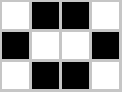
\includegraphics[height=.45\linewidth]{./images/beehive.png}
        \caption{}
        \label{fig:2-1}
    \end{subfigure}
    \quad
	\begin{subfigure}[b]{0.3\linewidth} 
        \centering
        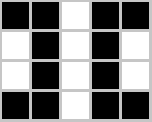
\includegraphics[height=.5\linewidth]{./images/table_on_table.png}
        \caption{}
        \label{fig:2-2}
    \end{subfigure}
	\\    
    \begin{subfigure}[b]{0.3\linewidth} 
        \centering
        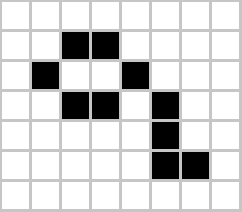
\includegraphics[height=0.5\linewidth]{./images/beehive_with_tail.png}
        \caption{}
        \label{fig:2-3}
    \end{subfigure}
    \quad
	\begin{subfigure}[b]{0.3\linewidth} 
        \centering
        
\includegraphics[height=.35\linewidth]{./images/biblock.png}
        \caption{}
        \label{fig:2-4}
    \end{subfigure}
	\caption{Algunas vidas inmóviles del juego de vida de Conway.}
	\label{fig:inmoviles}
\end{figure} 


Notar que pueden estar formadas a su vez por varias \textit{vida inmóvil} y que o bien dependan entre sí para mantener su estabilidad como en la \autoref{fig:2-3}, o bien sean independientes y al eliminar algunas de ellas la estabilidad se mantenga como en la \autoref{fig:2-4}. También existen \textit{vida inmóvil} que pueden ser separadas en vidas inmóviles independientes y que además existan nodos vacíos que tanto en la configuración inicial como en las \textit{vidas inmóviles} independientes se mantengan así. Un ejemplo de esta situación se pueden observar en \autoref{fig:bimoved}.

\begin{figure}[H]
	\centering
	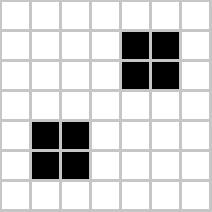
\includegraphics[height=.2\linewidth]{./images/bimoved.png}
	\caption{Configuración inicial que en el centro hay un nodo vacío que se mantiene tanto en las \textit{vidas inmóviles} independientes como en el total.}
	\label{fig:bimoved}
\end{figure} 

Por último, cabría preguntarse el problema de dado un número finito de nodos ocupados, ¿cuántas \textit{vidas inmóviles} existen? Dicho problema ha sido resuelto para \textit{vidas inmóviles} de hasta 32 nodos ocupados, como se puede consultar en \cite{countStillLifes}.

\subsection{Osciladores}

%\begin{defi}
%Un oscilador es una configuración inicial $z$ finita y no vacía que se repite tras la aplicación de $k$ veces de la función de transición global, esto es, fijado $n\in\mathds{N}$, se verifica que existe $k>1, \in\mathds{N}$ tal que $C^n_t(z) = C^n_{t+k}(z)$ para todo $t \leq n-k$ y diremos que $k$ es el periodo del oscilador.
%\end{defi}

Un \textit{oscilador} es una configuración inicial que tras un número fijo de iteraciones se repite en la misma posición, al número de iteraciones se le conoce por periodo del \textit{oscilador}. En particular, las vidas inmóviles pueden ser interpretadas como \textit{osciladores} de periodo una iteración.

En la \autoref{fig:congIniciales3} mostramos dos configuraciones iniciales de periodo dos, durante tres iteraciones. Por un lado la \autoref{fig:blinker1}, \autoref{fig:blinker2} y \autoref{fig:blinker3} son tres iteraciones de la configuración inicial nombrada \textit{blinker} y por otro la \autoref{fig:toad1}, \autoref{fig:toad2} y \autoref{fig:toad3} son tres iteraciones de la configuración inicial \textit{toad}.

\begin{figure}[H]
	\centering
	\begin{subfigure}[b]{0.3\linewidth} 
        \centering
        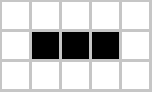
\includegraphics[height=.35\linewidth]{./images/blinker1.png}
        \caption{}
        \label{fig:blinker1}
    \end{subfigure}
    \ 
	\begin{subfigure}[b]{0.3\linewidth} 
        \centering
        
\includegraphics[height=.45\linewidth]{./images/blinker2.png}
        \caption{}
        \label{fig:blinker2}
    \end{subfigure}
    \ 	
    \begin{subfigure}[b]{0.3\linewidth} 
        \centering
        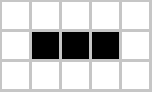
\includegraphics[height=.35\linewidth]{./images/blinker3.png}
        \caption{}
        \label{fig:blinker3}
    \end{subfigure}
    \\
	\begin{subfigure}[b]{0.3\linewidth} 
        \centering
        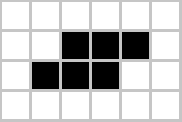
\includegraphics[height=0.35\linewidth]{./images/toad1.png}
        \caption{}
        \label{fig:toad1}
    \end{subfigure}
	\begin{subfigure}[b]{0.3\linewidth} 
        \centering
        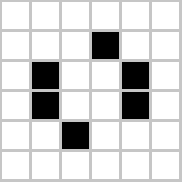
\includegraphics[height=0.45\linewidth]{./images/toad2.png}
        \caption{}
        \label{fig:toad2}
    \end{subfigure}
	\begin{subfigure}[b]{0.3\linewidth} 
        \centering
        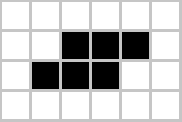
\includegraphics[height=0.35\linewidth]{./images/toad3.png}
        \caption{}
        \label{fig:toad3}
    \end{subfigure}
	\caption{Primeras 3 iteraciones de 2 \textit{osciladores} de periodo 2 del juego de vida de Conway.}
	\label{fig:congIniciales3}
\end{figure} 

\subsection{Naves espaciales} \label{spaceships}

%\begin{defi}
%Una  nave espacial es una configuración inicial $z$ finita y no vacía que se repite tras la aplicación de $k$ veces de la función de transición global pero en una posición distinta, esto es, fijado $n\in\mathds{N}$, se verifica que existen $k\in\mathds{N}$ y una traslación distinta de la identidad, $\phi:\mathds{Z}^2\to\mathds{Z}^2$, tal que $C^n_t(z) = \phi(C^n_{t+k}(z))$ para todo $t \leq n-k$ y diremos que $k$ es el periodo de la nave espacial.
%\end{defi}

Una \textit{nave espacial} es una configuración inicial es una configuración inicial que tras un número fijo de iteraciones se repite pero en una posición desplazada. Particularmente, pueden ser vistas como osciladores que en el periodo de oscilación se desplazan. Dado que este tipo de configuraciones iniciales se desplaza sobre la malla rectangular es interesante considerar la velocidad con la que lo hacen. Si una configuración inicial se desplaza $(x, y)$ unidades cada periodo de longitud $n$, la velocidad de desplazamiento de la nave espacial es: $$
 v = \frac{\max\{|x|,|y|\}}{k}
$$ 
y su pendiente es $x/y$.  $c$ es la velocidad máxima teórica, esto es, un desplazamiento por iteración. Curiosamente se ha probado que para cada pendiente existe una \textit{nave espacial} con dicha pendiente \cite{pendienteNaves}.

En la \autoref{fig:congIniciales4} encontramos dos \textit{naves espaciales} que se desplazan en distintas direcciones. La \autoref{fig:glider} es la \textit{nave espacial} más pequeña conocida de velocidad $c/4$ y su desplazamiento es diagonal y la \autoref{fig:lightweightspaceship} es la más pequeña conocida de velocidad $c/2$ y su desplazamiento es horizontal.

\begin{figure}[H]
	\centering
	\begin{subfigure}[b]{0.3\linewidth} 
        \centering
        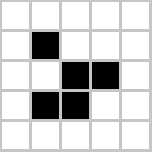
\includegraphics[height=.35\linewidth]{./images/glider.png}
        \caption{}
        \label{fig:glider}
    \end{subfigure}
    \quad
	\begin{subfigure}[b]{0.3\linewidth} 
        \centering
        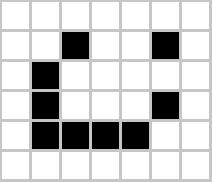
\includegraphics[height=0.45\linewidth]{./images/lightweightspaceship.png}
        \caption{}
        \label{fig:lightweightspaceship}
    \end{subfigure}
	\caption{Algunas \textit{naves espaciales} del juego de vida de Conway.}
	\label{fig:congIniciales4}
\end{figure} 


\subsection{Selección de configuraciones iniciales} \label{seleccion}

Los primeros censos de configuraciones iniciales fueron \textit{The Online Life-Life CA Soup Search} y \textit{Achim Flammenkamp's census}, en los que se contabilizaron 174.631.866.050 y 50.158.095.316 configuraciones del juego de vida, respectivamente. El primero de ellos consistió en la evolución de 6.412.048.029 configuraciones iniciales aleatorias que cubren un cuadrado de lado 20 con densidad inicial de 0.5 sobre una malla rectangular infinita \cite{sopa1}. El segundo exploró la evolución de 1.829.196 configuraciones iniciales aleatorias sobre una malla cuadrada de lado 2048 con los bordes opuestos identificados y con una densidad inicial de 0.375 \cite{sopa2}. De ambos censos se puede extraer la conclusión de que las configuraciones que aparecen más a menudo son las vidas inmóviles, seguidas por los osciladores y por último las naves espaciales.

Para nuestro trabajo tomaremos de referencia el censo más actual \textit{Catalogue} que recoge las ejecuciones de 19.640.649.096.999 configuraciones iniciales aleatorias cuadradas de lado 16 del juego de vida de Conway. Se han obtenido un total de 429.049.899.985.558 patrones de los cuales se encontraron 161.861 tipos diferentes \cite{sopa3}. En la tabla \autoref{tab:sopa1naves} se muestran las primeras 5 naves espaciales más frecuentes, las cuales escogeremos para realizar nuestro experimento. Destacar que todas son de periodo 4 y que no tomaremos más dado que el número de ocurrencias disminuye drásticamente de la cuarta a la quitan posición. En la \autoref{fig:congIniciales5} podemos observar la forma de estas configuraciones iniciales. Como representantes de la categoría de osciladores estudiaremos los dos osciladores más frecuente de periodo 2, 3 y 4. [Sin concretar porque está sujeto a cambios]

\begin{table}[]
\centering
\begin{tabular}{|l|l|l|l|}
\hline
Ranking & Nombre                          & Periodo & Ocurrencias    \\ \hline
1       & \textit{Glider}                 & 4       & 37.699.263.597.381 \\ \hline
2       & \textit{Lightweight spaceship}  & 4       & 55.075.316.989     \\ \hline
3       & \textit{Middleweight spaceship} & 4       & 14.511.262.233      \\ \hline
4       & \textit{Heavyweight spaceship}  & 4       & 2.521.819.486      \\ \hline
5       & \textit{MWSS on MWSS}  & 4       & 7.077      \\ \hline
\end{tabular}
\caption{Naves espaciales más frecuentes}
\label{tab:sopa1naves}
\end{table}

\begin{figure}[H]
	\centering
	\begin{subfigure}[b]{0.3\linewidth} 
        \centering
        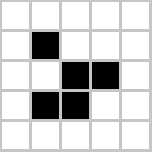
\includegraphics[height=.45\linewidth]{./images/glider.png}
        \caption{\textit{Glider}}
        \label{fig:glider}
    \end{subfigure}
    \ 
	\begin{subfigure}[b]{0.3\linewidth} 
        \centering
        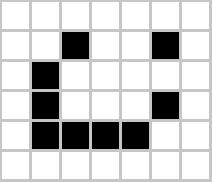
\includegraphics[height=0.45\linewidth]{./images/lightweightspaceship.png}
        \caption{\textit{Lightweight spaceship}}
        \label{fig:lightweightspaceship}
    \end{subfigure}
    \
	\begin{subfigure}[b]{0.3\linewidth} 
        \centering
        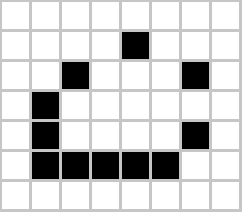
\includegraphics[height=0.45\linewidth]{./images/middleweightspaceship.png}
        \caption{\textit{Middleweight spaceship}}
        \label{fig:middleweightspaceship}
    \end{subfigure}
    \\
	\begin{subfigure}[b]{0.3\linewidth} 
        \centering
        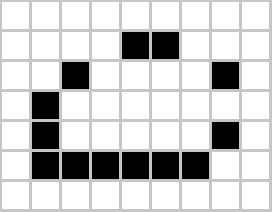
\includegraphics[height=0.45\linewidth]{./images/heavyweightspaceship.png}
        \caption{\textit{Heavyweight spaceship}}
        \label{fig:heavyweightspaceship}
    \end{subfigure}
    \
	\begin{subfigure}[b]{0.3\linewidth} 
        \centering
        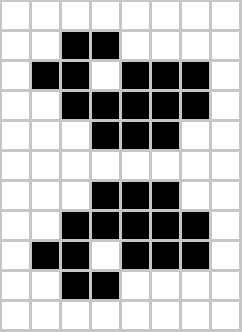
\includegraphics[height=0.65\linewidth]{./images/MWSS_on_MWSS.png}
        \caption{\textit{MWSS on MWSS}}
        \label{fig:mwss2}
    \end{subfigure}
	\caption{Top 5 naves espaciales más frecuentes en el censo {Catalogue}.}
	\label{fig:congIniciales5}
\end{figure} 


% aquí hay que exponer que se descartan las vidas inmóviles porque no se ven afectadas por la perturbación de la actualización

\section{Simulaciones} \label{vars}

Dado el carácter aleatorio del juego de vida $\alpha$-asíncrono emplearemos los fundamentos de Monte Carlo expuestos en la sección \ref{MonteCarlo} para medir los parámetros de interés que a continuación exponemos. Nuestras variables de interés son:

\begin{itemize}
\item Crecimiento de la población de células de la configuración inicial: dispondremos de dos herramientas para medir el número de células. Estudiaremos la evolución del número de células en cada etapa, la evolución del área del rectángulo de menor tamaño que contenga a todas las células de cada etapa y su densidad, esto es, el cociente del número de células entre el área anterior.
\item Tasa de cambio de la configuración inicial: emplearemos el concepto de calor, el número de células que nacen o mueren por generación.
\item Distribución de las células en cúmulos: contabilizaremos el número de cúmulos por cada generación, entendiendo por cúmulo al mayor conjunto de células cuyo vecindario no es disjunto, es decir, en un cúmulo cada célula está contenida en el vecindario de otra célula del cúmulo.
\end{itemize}

Estas variables serán medidas para distintos valores de $\alpha$ con el fin de estudiar el efecto de la aleatoriedad en las configuraciones iniciales. Notar que el número de simulaciones realizadas para cada patrón será variable puesto que algunos patrones son de mayor tamaño y en consecuencia tienen simulaciones más lentas.

% Características a medir si sobra tiempo: simulaciones utilizando cadenas de markov y métodos de monte carlo



\end{document}
